\documentclass[conference]{IEEEtran}
\usepackage{amsmath,amsfonts,amssymb}
\usepackage{graphicx}
\usepackage{listing}
\usepackage{subfig}
\usepackage{color}
\usepackage{url}

%\usepackage{url}

\begin{document}
\title{CS8803-O03 Reinforcement learning\\Project 3 report}

\author{\IEEEauthorblockN{Rohan D. Kekatpure}
\IEEEauthorblockA{Email: rdk@gatech.edu}}
% make the title area
\maketitle

% As a general rule, do not put math, special symbols or citations
% in the abstract
%\begin{abstract}
%\end{abstract}

\IEEEpeerreviewmaketitle
\section{Introduction}
Multi-agent Q-learning is a nontrivial departure from deterministic action, single $Q$ function MDPs in two ways: (1) state values are functions of multiple Q's (2) optimal policies are allowed to be stochastic. The Greenwald paper \cite{greenwald} demonstrates the inadequacy of regular Q learning and convergence of multi-agent Q learning learning. Project 3 aims to deepen our understanding of multi-agent (adversarial or cooperative) Q learning through reproduction of Greenwald's results for a $2\times4$ grid game called soccer.

%%
\section{Quick theory tour}
The paper presents four multi-agent Q learning options:
\begin{enumerate}
\item {\bf Q learning:} Ignore the opponent's $Q$ function and actions. Agents are only coupled through rewards. The policy is deterministic and $Q$ function at each state for each agent is simply a vector of $n$ values ($n=5$ in our case). The state value is the max for $Q_i$: 
\begin{equation}
V_i =\max_{a\in A_i} Q_i(s,a)
\end{equation} 
%
\item {\bf Friend Q: } Ignore the opponent's $Q$ function, but consider its actions. Optimal policy is deterministic, and $Q$ function at each stage is a $n\times n$ matrix. The value for each state is the max across this matrix:
\begin{equation}
V_i = \max_{\vec{a}\in A_1\times A_2} Q_i(s, \vec{a})
\end{equation}
%
\item {\bf Foe Q: } Ignore opponent $Q$ function, consider its actions, but calculate the value function using {\bf maximin} instead of simple max. This requires linear programming (LP). Maximin also allows {\bf stochastic} optimal policies represented as a probability distribution over $n$ action values. The $Q$ is an $n\times n$ matrix and the state value is: 
%
\begin{equation}
V_i = \max_{\pi\in\text{PD}(A)}\min_{o\in O}\sum_{a\in A_i}\pi(a) Q_i(s, a, o)
\end{equation}
%
\item {\bf CE Q: } Consider joint actions and compute state value as a function of agents' $Q$ values
%
\begin{equation}
V_i = \sum_{\vec{a}\in A_1\times A_2} \sigma(\vec{a})Q_i(s, \vec{a})
\end{equation}
where $\sigma$ is a probability distribution over the $n^2$ action pairs computed using the {\em u}CE-Q objective out of the four CE options provided. In simplified notation:
\begin{equation}
\sigma = \arg \max_{\sigma\in\text{CE}} \sum_{\vec{a}\in A_1 \times A_2} \big[Q_1(s, \vec{a}) + Q_2(s, \vec{a})\big]
\end{equation}
\end{enumerate}
%%
\section{Implementation}
\subsection{Game representation}
The soccer world is a $2\times 4$ grid with row index $r\in [1,2]$ and column index $c\in [1,2,3,4]$. The state of the game is represented as:
\begin{equation}
s \stackrel{\Delta}{=} \text{tuple}((r_A,c_A), (r_B,c_B), \text{ball})
\end{equation}
The individual action space is $A_1, A_2 \in [N, W, E, S, T]$ ($T=$ stick) and the joint action space is $A_1\times A_2$. Since the number of states $ = 8\times 7\times 2 = 112$ is small, the Q values can be maintained in memory as a nested dictionary:
\begin{equation}
Q \stackrel{\Delta}{=} \{s: \{\vec{a}: (Q_A, Q_B)\}\} 
\end{equation}
where the inner dictionary maps 25 action pairs to a tuple of Q values for agents $A$ and $B$, and the outer dictionary maps this structure to the state. The structure can also be thought as a mapping from each of the 112 states to a $5\times 5\times 2$ matrix of Q values for $A$ and $B$ for each action pair. 
%%
\subsection{Simulation}
A {\bf move} is defined as one action each by $A$ and $B$ carried out in a random order. An {\bf episode} is a set of moves until a goal is scored. An episode can: (1) in theory continue forever and (2) end mid-move if a goal is scored.

To simulate a move, we select an action pair $(a_1, a_2)$ from $A_1\times A_2$ and assign it to $(A, B)$, who execute in random order. After executing its action, each agent checks for the game-end condition and receives rewards for reaching the next state. Rewards are zero except when the game ends. In addition to the prescribed rules, we observed the following additional conventions: (1) an episode never starts in the end condition, (2) goal is counted even when a stationary empty-handed agent in a goal position is handed a ball by the mobile ball-carrying agent; i.e. $A$ could lose if it is in $B$'s goal position and handed a ball.

After each move, values $V_i$, $i\in [A,B]$ for each state are calculated and used to update the two $Q$-functions according to the update equations in Table 1 in the Greenwald paper. Because of the small number of states, we learn via an {\bf off-policy} $Q$ learning algorithm (i.e. actions are always random).
%%
\subsection{Recording $Q$-function difference}
The paper reports the evolution of the $Q_A$ values for the state $s = ((1, 3)_A,(1,2)_B, B)$ (a.k.a the monitor state) for the action pair $ST$. The evolution of the $Q$ values for the monitor state are stored in an array and updated only when that state is actually encountered in an episode. A global timestep counter, which increments across episodes, is maintained to record the value of the timesteps at which the monitor state is updated. The $Q$-function difference is calculated exactly according to the prescription: $\textsc{err}_A^t = \vert Q_A^t(s, \vec{a}) - Q_A^{t-1}(s, \vec{a})\vert$.
\subsection{Linear programming}
Correlated Q and Foe Q implementation require LP. After some research \cite{cvxopt}, we chose the {\tt CVXOPT} LP package with the GNU {\tt glpk} solver. This resulted in over $10\times$ speedup relative to {\tt PuLP}, {\tt SciPy} and {\tt CVXOPT}'s default solver. However, setting up the problem in {\tt CVXOPT}'s matrix language requires care (proper negations, column ordering etc).
\subsection{Software dependencies}
The only external packages for our implementation are {\tt CVXOPT}, {\tt numpy} for core computation and {\tt matplotlib} and {\tt Pandas} for postprocessing.
\subsection{Hyperparameters}
We experienced that the convergence curves are {extremely sensitive} to the choice of initial learning rate and the decay schedule. We've collected the hyperparemeters of our implementation in Table~\ref{tab:hyper}.
\begin{table}[!h]
\begin{center}
\begin{tabular}{|l|l|}
\hline
Hyperparameter & Value\\ \hline 
Discount $\gamma$ & 0.9\\
Decay schedule & $\alpha = \max(\alpha_{\text{min}}, \alpha_0\alpha_d^t$) \\
$\alpha_0$ & 0.15 \\
$\alpha_{\text{min}}$ & $10^{-3}$ \\ 
$\alpha_d$ & 0.9999954 \\ \hline
\end{tabular}
\end{center}
\caption{Hyperparameters for all $Q$-learning algorithms. \label{tab:hyper}}
\end{table}
%%
\section{Results}
The results of the simulation of the soccer game are displayed in Fig.~\ref{fig:maql}. We start our description with Fig.~\ref{fig:maql}(d), which shows the results for regular (or un 
%
\begin{figure*}[htbp]
\centering 
\begin{tabular}{cc}
    \subfloat[CE-Q] {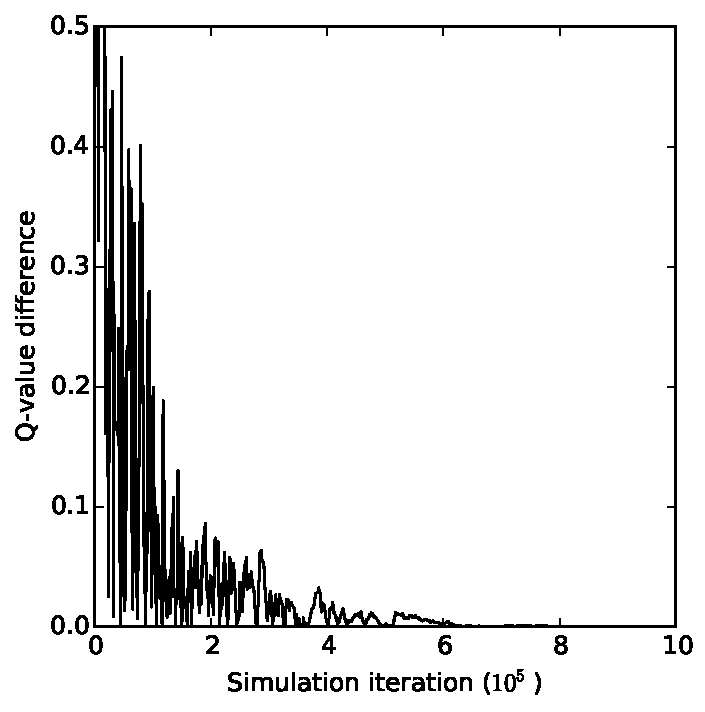
\includegraphics[width=0.4\textwidth]{./figures/ceq.pdf}} 
    & \subfloat[Foe-Q] {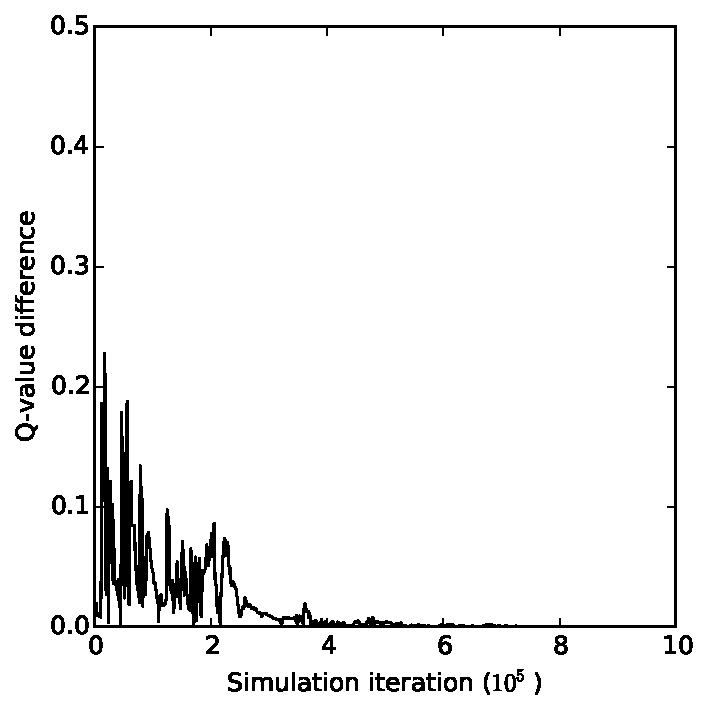
\includegraphics[width=0.4\textwidth]{./figures/foe.pdf}} \\
    \subfloat[Friend-Q] {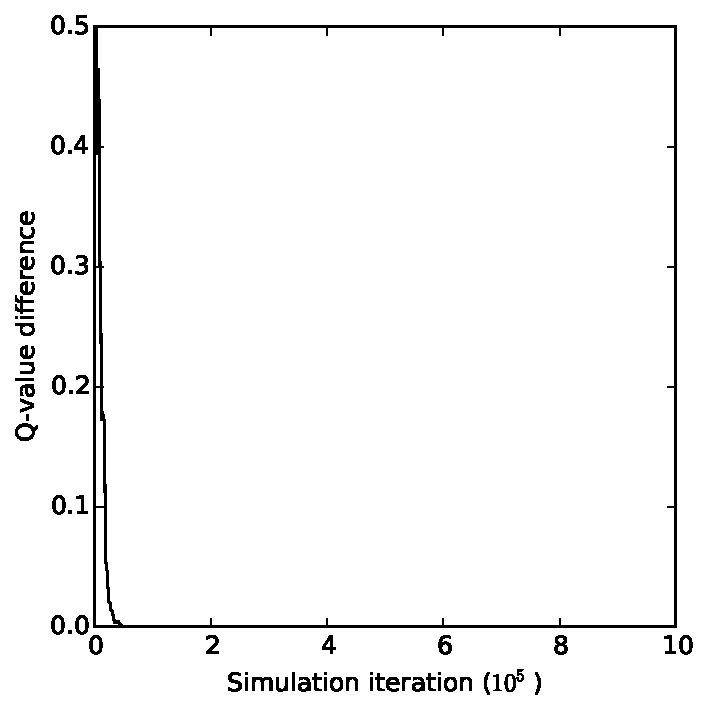
\includegraphics[width=0.4\textwidth]{./figures/friend.pdf}}
    & \subfloat[Q-learning] {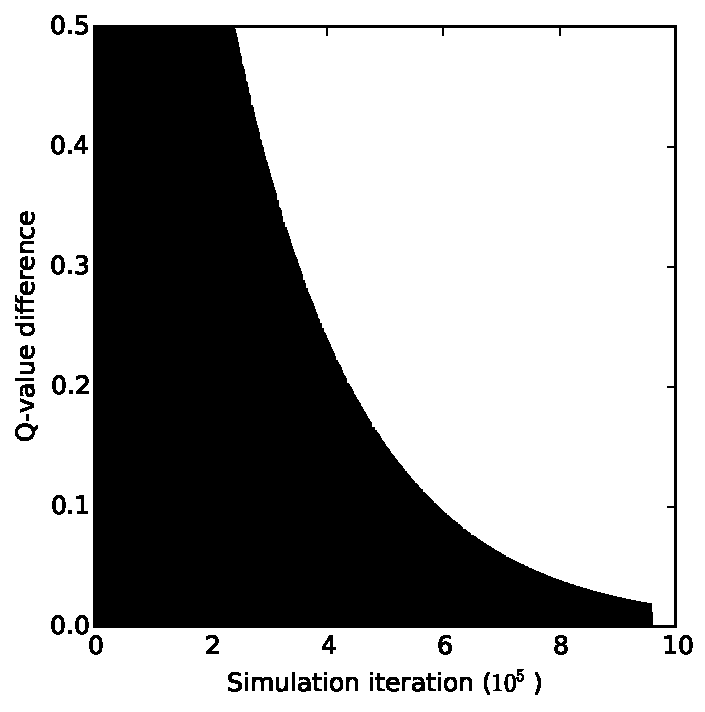
\includegraphics[width=0.4\textwidth]{./figures/qlearning.pdf}}    
\end{tabular}
\caption{Results of the soccer game in the Greenwald paper. (a) Correlated $Q$, (b) Foe $Q$, (c) Friend $Q$ and (d) $Q$ learning.\label{fig:maql}}
\end{figure*}
%%
\section*{Summary}
\begin{thebibliography}{1}
\bibitem{greenwald}
A.~Greenwald and K.~Hall, ``Correlated Q learning,'' {\em ICML}, 2001.
\bibitem{cvxopt}
S.~Caron,``Linear Programming in Python with CVXOPT,'' {\em \url {https://scaron.info/blog/linear-programming-in-python-with-cvxopt.html}}
\end{thebibliography}

\end{document}


